\documentclass[12pt, letterpaper]{article}
\usepackage[a4paper,left=3cm,right=2cm,top=2.5cm,bottom=2.5cm]{geometry}

\usepackage[utf8]{inputenc}
\usepackage{graphicx}
\graphicspath{ {images/} }
\usepackage{amsmath,bm}
\usepackage{listings}
\usepackage{float}


\title{4TN4 Assignment 1}
\author{Adam Bujak}
\date{January 21, 2022}

\begin{document}

\maketitle

\section{Theory}

\subsection{Phone Camera Parameters}

\begin{figure}[h]
    \centering
    \includegraphics[width=.8\textwidth]{phone}
    \caption{Phone Specifications}
    \label{fig:phone}
\end{figure}

\subsubsection{Resolution}

\textbf{What does the camera resolution show?}

The main camera (wide) is a 50MP camera - indicating that there are 50 million pixels. This is simply a measure of how many RGB measurements are recorded for each photograph.

\subsubsection{Sensor Size}

\textbf{As shown the size of the main camera is 2.44\textmu m while the selfie camera sensor size is 0.8\textmu m. First define the
camera sensor size and the state what is the advantage of having larger sensor size?}

The 2.44\textmu m measurement refers to the size of each individual pixel's size. The advantage of having a larger sensor is that you have more light sensing area per each pixel, therefore, you can capture more light, and more importantly, reduce the noise in the light measurement on a per pixel basis.

\subsubsection{PDAF}

\textbf{What does PDAF stand for? Explain shortly how it works?}

PDAF stands for \textit{Phase Detection Autofocus} which works by splitting the image into two phases using prisms, and then adjusting the lens until the two phases are in sync - this is when the image is in focus.

\subsubsection{Shutter Speed}
\textbf{What is shutter speed? What do we lose and gain when we take a photo using high shutter speed?}

Shutter speed is defined by how quickly the shutter opens and closes. Perhaps a more intuitive and practical term for this is \textit{exposure time}, especially in modern times where more and more cameras do not have a physical shutter. Exposure time is the time for which sensor readings are made during an exposure (taking a photograph). Longer exposure times increase the time of exposure and increase the amount of light available for measurement. However, in well lit environments too long of an exposure will result in burn in (the imaging equivalent of audio clipping), since the maximum sensor reading will be reached. Too long of an exposure will also result in motion blur if objects in the scene are moving. Too short of an exposure time (high shutter speed) will result in not as much light being available for measurement and may result in an under-exposed image, however, a higher shutter speed will result in less motion blur and therefore a sharper image if the environment is in motion.

\subsubsection{OIS}
\textbf{What does OIS stand for? Using OIS, we can use a lower shutter speed. How could this improve the quality of
the taken image?}

OIS stands for \textit{Optical Image Stabilization}. Camera systems that use OIS physically stabilize either the sensor or the lens which reduces the motion blur effect due to the camera system shaking while being operated. By reducing the movement of the image on the sensor, we can get a clearer, sharper image at slower shutter speeds.

\subsubsection{ISO}
\textbf{What is ISO sensitivity in cameras?}

ISO sensitivity essentially determines the gain for amplifying the light readings. A high ISO will result in a brighter image but higher noise levels. A low ISO will result in a dimmer image (thus requiring longer exposure times) but a much clearer image with less noise.

\subsection{Gamma Correction}
\textbf{Why gamma correction is useful? present the formula of gamma correction and plot the output value vs. input
value (assume the images are between 0 and 255) for $\gamma = \{0.25,0.5,1,1.5,2\}$}

Camera sensors are linear - when two units of light hit the sensor, the pixel will be twice as bright as when one unit of light hits the sensor. This is not always the case in humans. Especially in darker scenarios where humans are much more sensitive to changes in brightness. Gamma correction corrects for this with the following formula, where $P$ is a given pixel value.

\[ P' =  (\frac{P}{255}) ^ {\frac{1}{\gamma}} \cdot 255\]

\vspace{.5cm}

\begin{figure}[h]
    \centering
    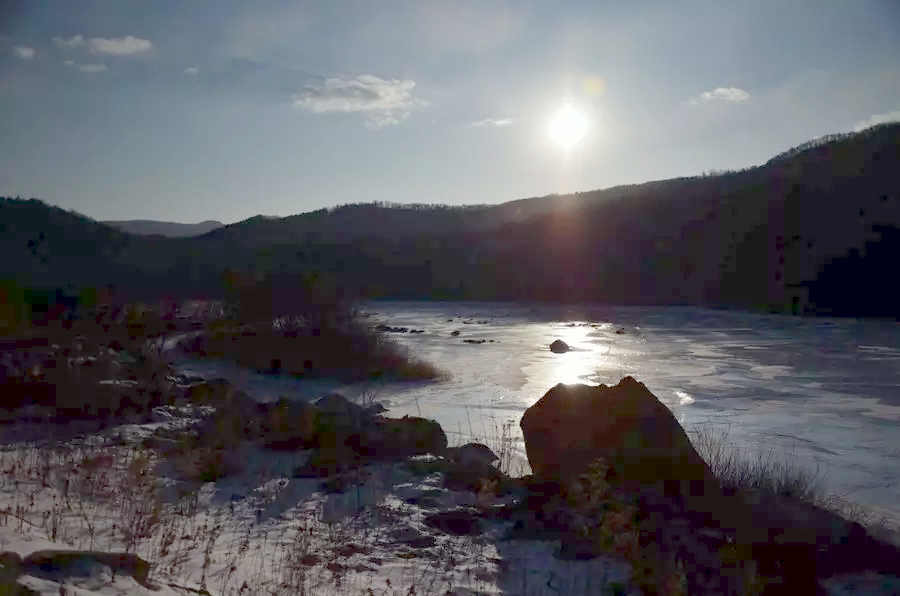
\includegraphics[width=\textwidth]{gamma_correction.png}
    \caption{Gamma Correction with varied gamma values}
    \label{fig:gamma}
\end{figure}

\subsection{Colour Spaces}
\textbf{What is XYZ and XYy color spaces? Explain what is chromaticity diagram and plot it.}

\subsubsection{XYZ}

XYZ colour space is the representation of all possible colours the average human can see (experimentally observed by varying test colour wavelength) where X, Y, and Z correspond to light functions that are purely theoretical. When researchers attempted to recreate colours of certain wavelengths using real red, green, and blue colours, they found that they had to "subtract" certain colours to recreate the test colour. To avoid the "subtraction" of light, which is impossible, they developed the XYZ basis which avoids this issue, by allowing the recreation of any colour through pure addition.


\subsubsection{xyY}

xyY is the normalized version of XYZ where the x and y are defined by the following equations, and Y remains the same to represent only luminance. Therefore, x and y completely represent the chromaticity of a colour, and Y represents the luminance.

\[ x =  \frac{X}{X+Y+Z}\]
\[ y =  \frac{Y}{X+Y+Z}\]

\subsubsection{What is a chromaticity diagram?}

The chromaticity diagram of the CIE 1931 (XYZ) colour space is a visual representation of all of the colours visible to the average human. One can observe all of the possible colours that can be achieved by mixing two colours by connecting the two colours with a straight line. This further allows one to easily see how any colour can be created in an infinite number of ways, because as long as the path between the two colours used passes through the desired colour, it is a possible combination to recreate the desired colour.

\begin{figure}[h]
    \centering
    \includegraphics[width=0.5\textwidth]{chrom.png}
    \caption{Chromaticity Diagram of the CIE 1931 (XYZ) colour space}
    \label{fig:chromaticity}
\end{figure}

\subsection{Interpolation}
\textbf{What is bilinear interpolation? How can it be used to upscale (upsample) an image?}

Linear interpolation is the process of estimating a value between two samples by drawing a straight line between the two samples and taking the value of the line at the time of interest. For instance if we know a drone was 5m above the ground at $t = 0s$ and 10m above the ground at $t = 2s$, we can estimate that the drone was 7.5m above the ground at $t=1s$.

Bilinear interpolation is the same idea but elevated into two dimensions. One way we can perform bilinear interpolation is by performing linear interpolation in one dimension first, and then using the values of the first interpolation, use linear interpolation again in the second dimension.

Bilinear interpolation can be used to upsample an image by adding more pixels by performing bilinear interpolation on the surrounding pixels. This would provide an estimate for the surrounding pixels, and will increase the resolution of the image. However, these extra pixels are only estimates, and are no replacement for a higher resolution original image.



\noindent{\textbf{Use bilinear interpolation to derive the green pixel value. (Q11 = 10,Q12 = 100,Q21 = 60,Q22 = 70)}}



\begin{figure}[h]
    \centering
    \includegraphics[width=0.35\textwidth]{bilinear.png}
    \caption{Bilinear Example Problem}
    \label{fig:bilinear}
\end{figure}


\noindent{\bm{$x_1=10, x=20, x_2= 50, y_1= 10, y=30, y_2= 40$}}

To find $P$ using bilinear interpolation, we can find $R_1$ and $R_2$, using linear interpolation, and then linearly interpolate between $R_1$ and $R_2$.

\[R_1 = \frac{Q_{21} - Q_{11}}{x_2-x_1} \cdot (x - x_1)  \]
\[R_2 = \frac{Q_{22} - Q_{12}}{x_2-x_1} \cdot (x - x_1)  \]

\[P = \frac{R_2 - R_1}{y_2-y_1} \cdot (y - y_1)  \]

\noindent{By plugging in, we find $R_1 = 12.5$, $R_2 = -7.5$, and $P=-13.\overline{3}$.}

\section{Implementation}

\subsection{Hello OpenCV}

\subsubsection{Code Screenshot}
\begin{figure}[H]
    \centering
    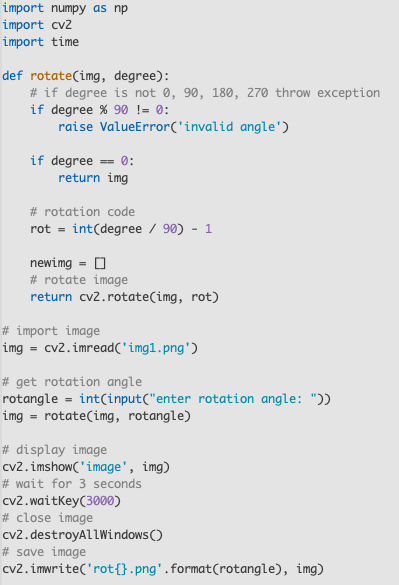
\includegraphics[width=\textwidth]{q1_screenshot.png}
    \caption{Hello OpenCV Python Code}
\end{figure}

\subsubsection{Results}

\begin{figure}[H]
    \centering
    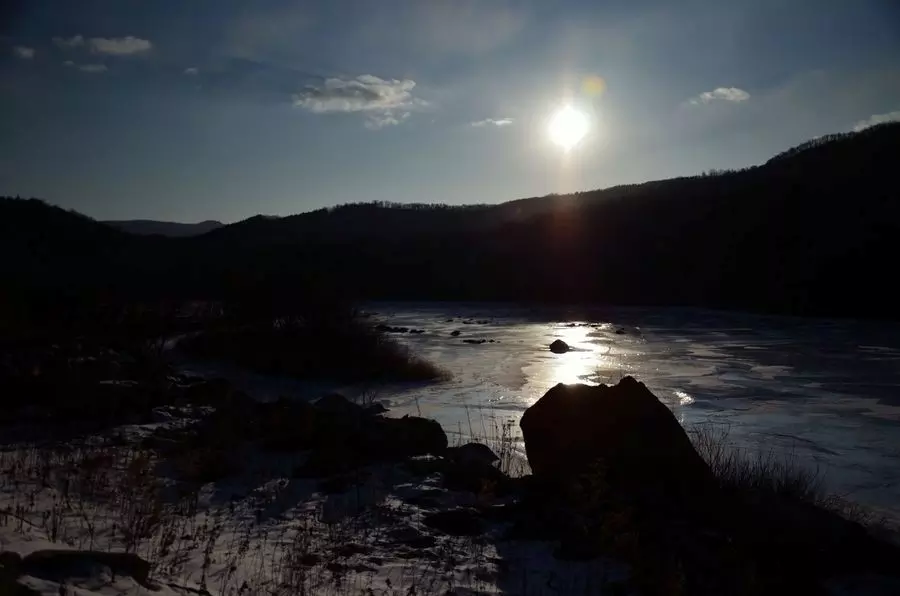
\includegraphics[width=0.5\textwidth]{rot0.png}
    \caption{0 Rotation}
\end{figure}

\begin{figure}[H]
    \centering
    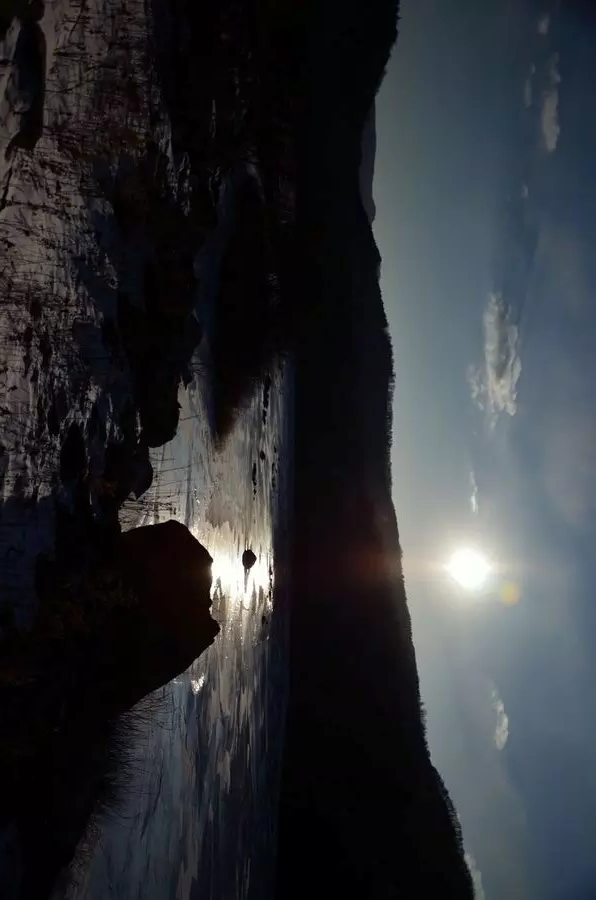
\includegraphics[width=0.5\textwidth]{rot90.png}
    \caption{90 Rotation}
\end{figure}

\begin{figure}[H]
    \centering
    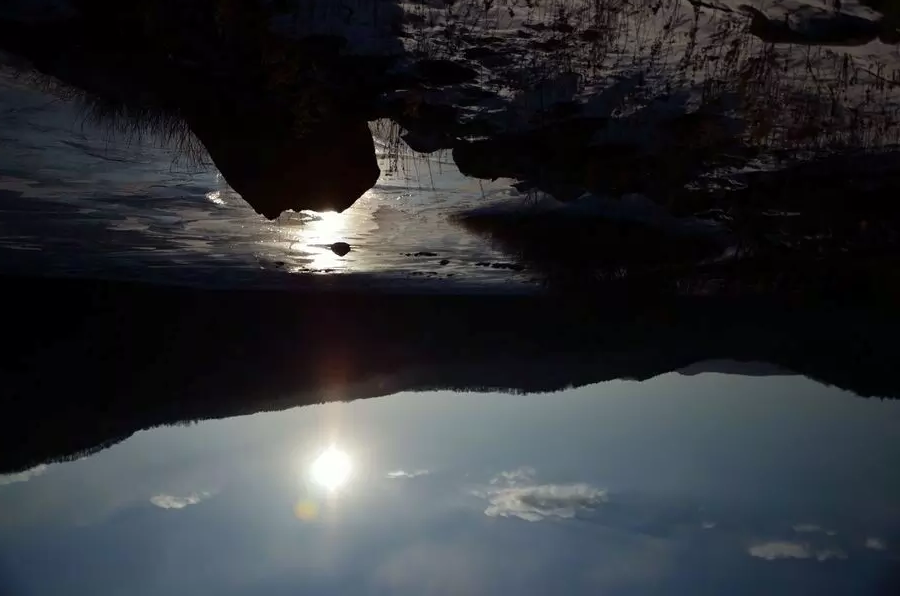
\includegraphics[width=0.5\textwidth]{rot180.png}
    \caption{180 Rotation}
\end{figure}

\begin{figure}[H]
    \centering
    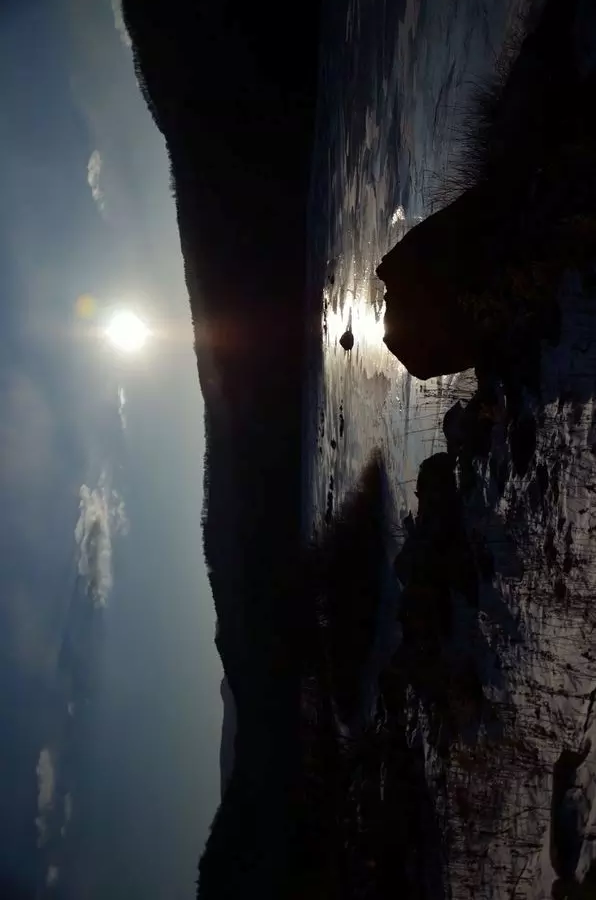
\includegraphics[width=0.5\textwidth]{rot270.png}
    \caption{270 Rotation}
\end{figure}

\subsection{Gamma Correction}

\subsubsection{Code Screenshot}
\begin{figure}[H]
    \centering
    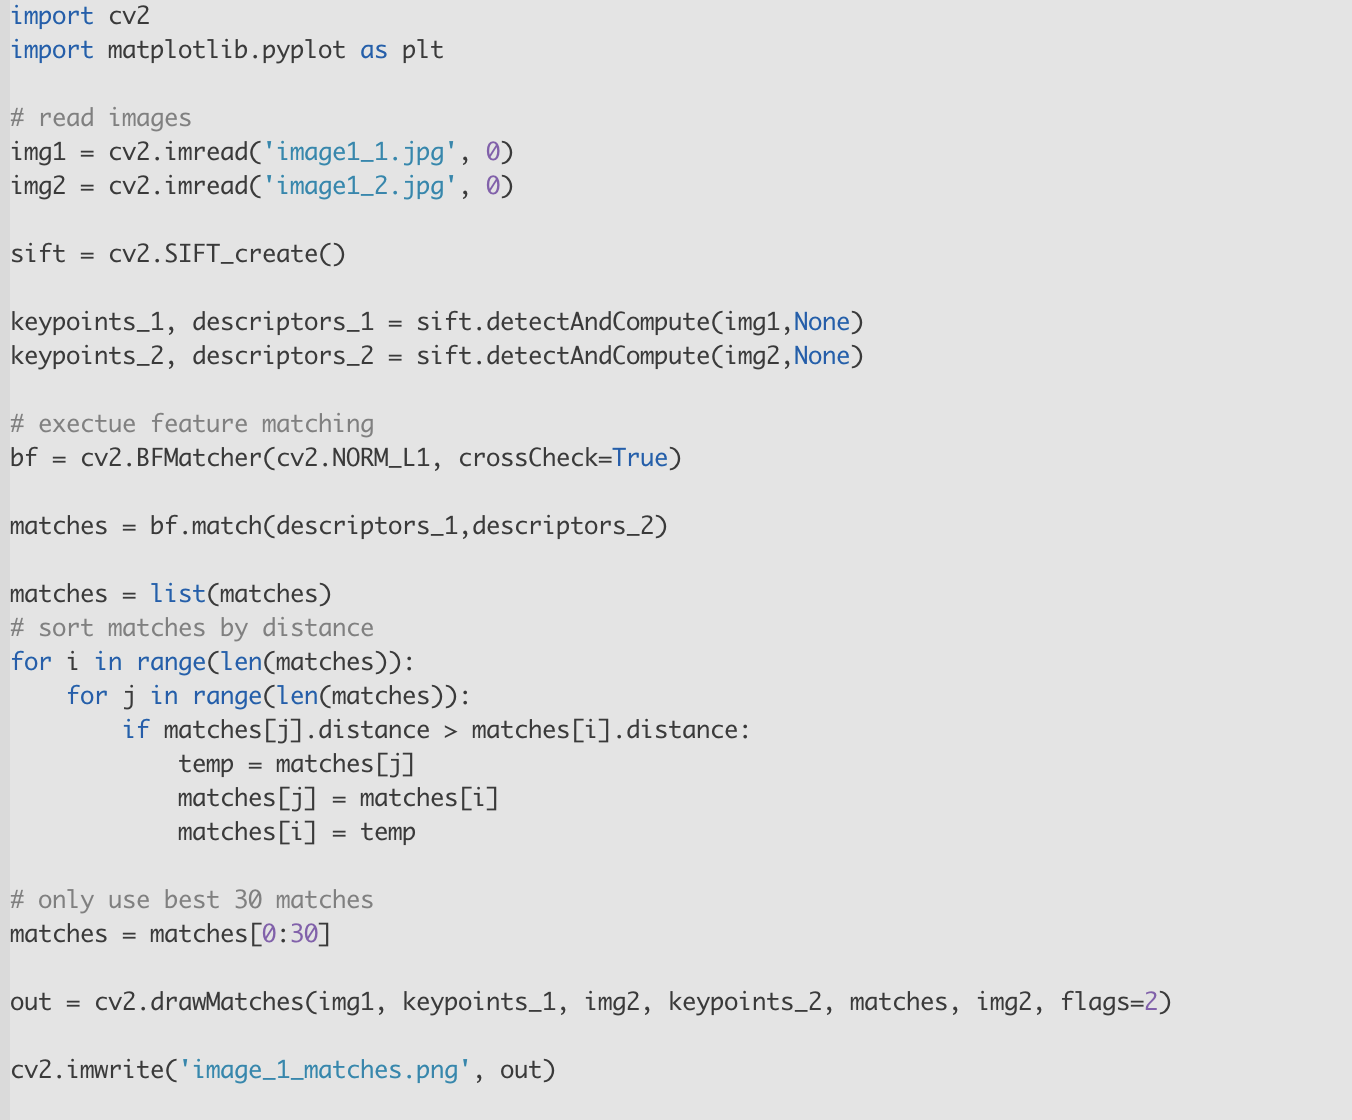
\includegraphics[width=\textwidth]{q2.png}
    \caption{Gamma Correction Python Code}
\end{figure}

\subsubsection{Results}


\begin{figure}[H]
    \centering
    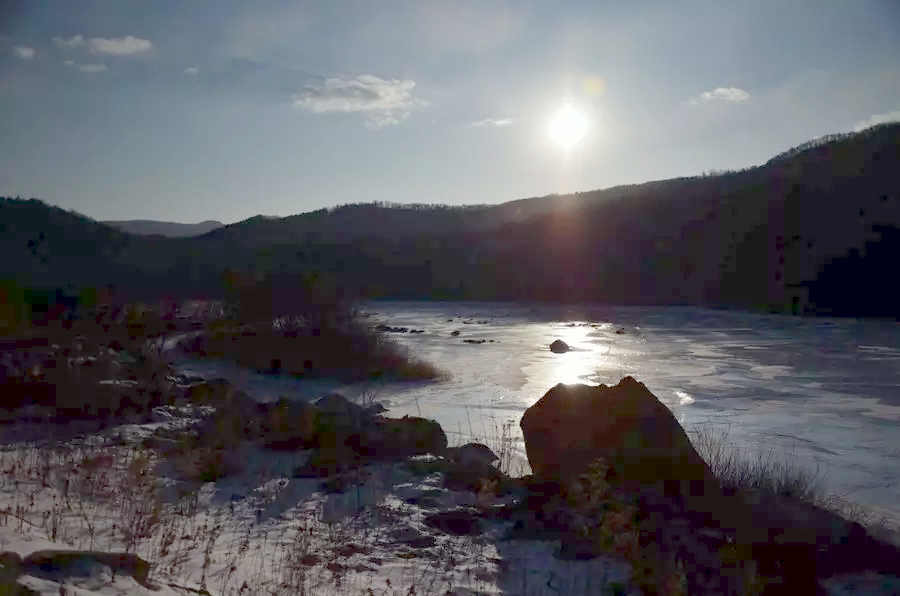
\includegraphics[width=0.5\textwidth]{gamma_correction_ex.png}
    \caption{Gamma Corrected image with $\gamma = 2$}
\end{figure}

\subsection{Skin Detection}

\subsubsection{Code Screenshot}
\begin{figure}[H]
    \centering
    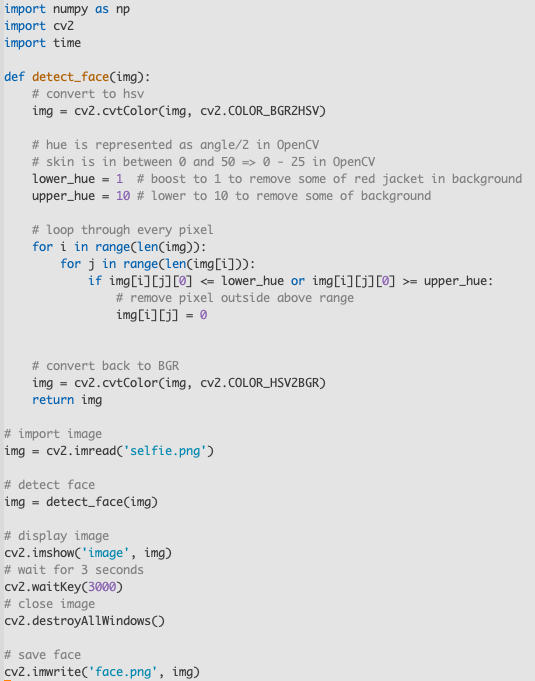
\includegraphics[width=\textwidth]{q3_screenshot.png}
    \caption{Skin Detection Python Code}
\end{figure}

\subsubsection{Results}

\begin{figure}[H]
    \centering
    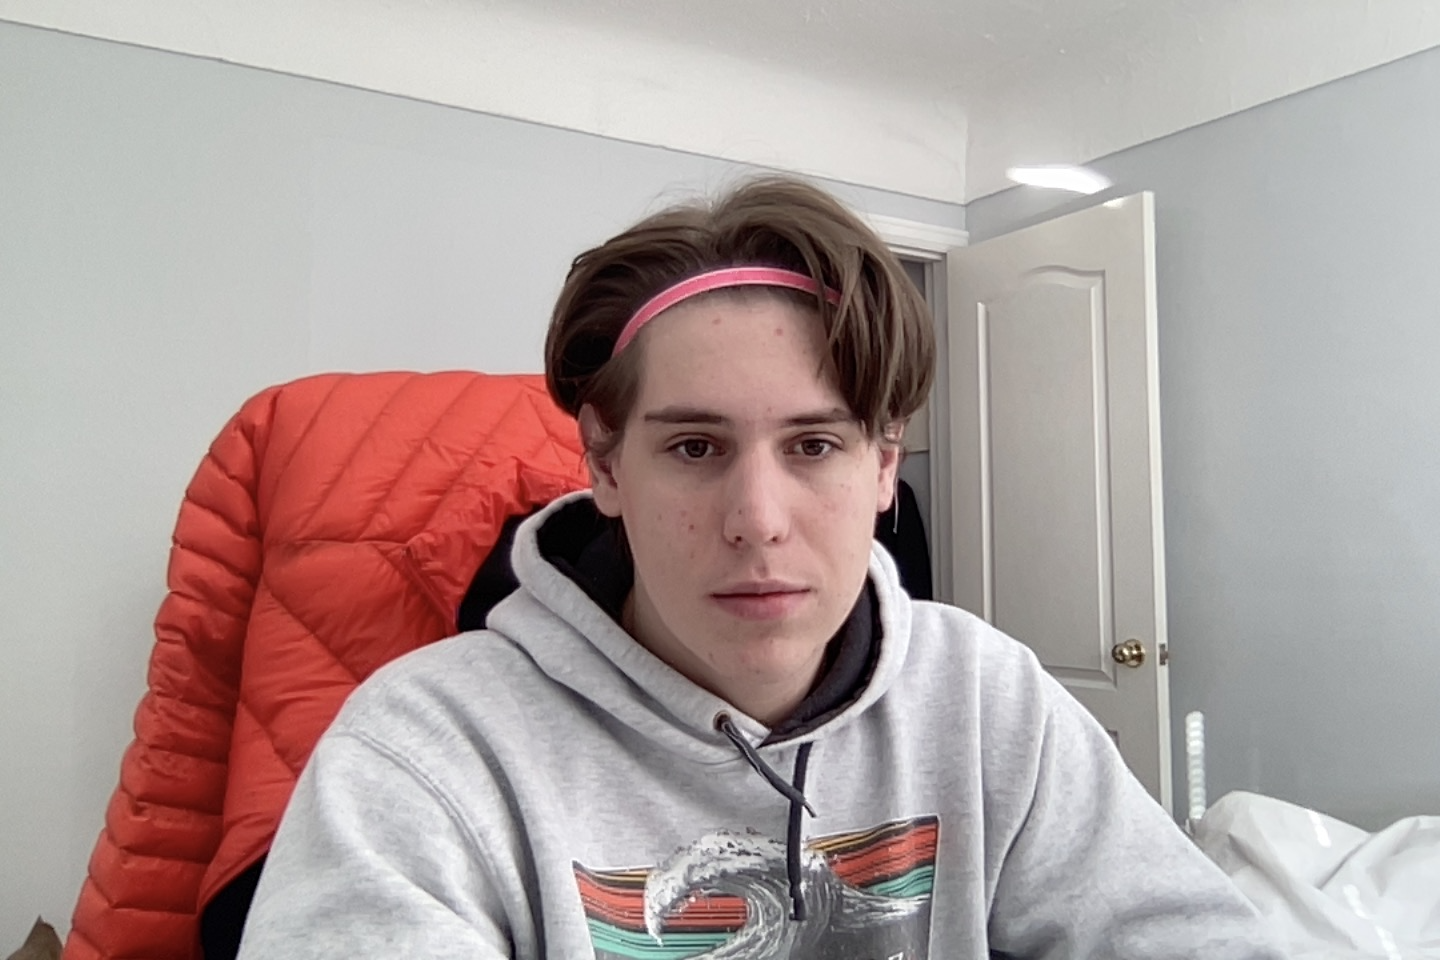
\includegraphics[width=0.5\textwidth]{selfie.png}
    \caption{Original Image}
\end{figure}

\begin{figure}[H]
    \centering
    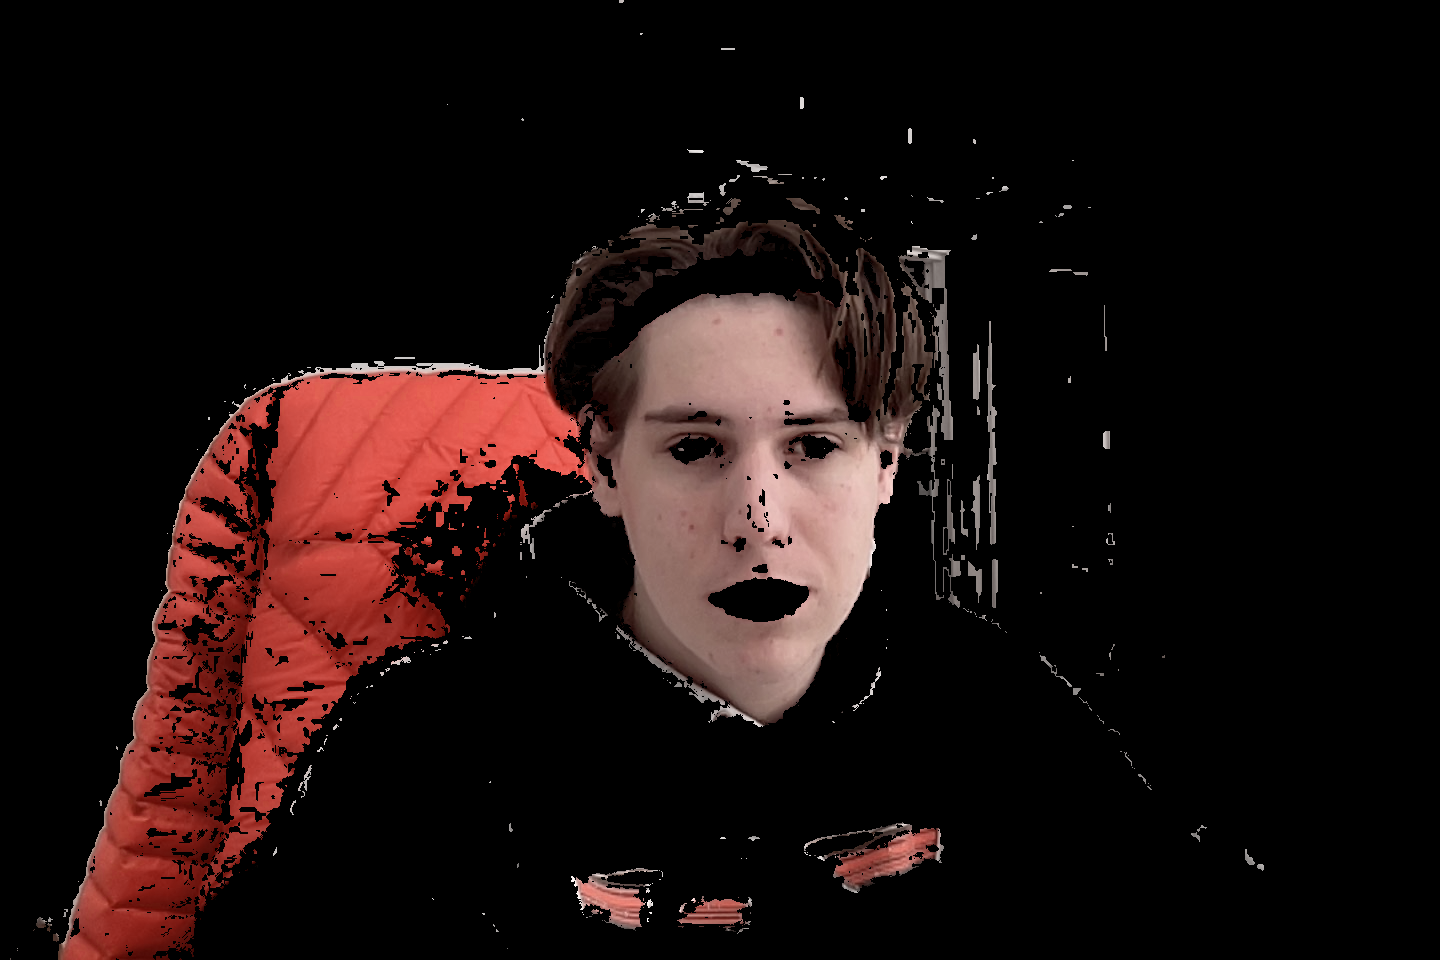
\includegraphics[width=0.5\textwidth]{face.png}
    \caption{Image outputted from skin detection}
\end{figure}



\end{document}
